% !TEX root = Séquence 2 - Cours - Vecteurs.tex
% Cours de la Séquence 2, copie indépendante du chapitre B1 du polycopié
% général (TeX - Polycopié et Exercices/Chapitres/Géométrie1_Vecteurs.tex),
% pour pouvoir l'adapter ici (ex. version élève à trous, comme la Séquence 1)
% sans toucher au polycopié. Recharge CLT2627.sty pour garder le rendu
% identique (boîtes Dfn/Prp/Exemple/Attention, puce cursive) du poly ;
% le titre reprend en revanche le bandeau \SequenceTitre de "Séquence 1 -
% Cours - Calculs Numériques.tex" plutôt que le bandeau-chapitre du poly.
\documentclass[a4paper,11pt,french]{report}
% \usepackage ne peut pas prendre un chemin contenant des espaces : LaTeX
% coupe les espaces internes du nom de paquet (\zap@space, pensé pour les
% listes "pkg1, pkg2"). On charge donc CLT2627.sty par \input direct, qui
% lui n'altère pas le nom de fichier.
\input{CLT2627.sty}
\graphicspath{{../TeX - Polycopié et Exercices/}}
\geometry{footskip=0.5cm}

% Croix de placement des points sur quadrillage (reprise de "Séquence 2 -
% Feuille d'exercices - Vecteurs.tex"), pour l'Exemple 2 (au lieu d'un
% point plein) : shapes.misc (cross out) déjà chargée par CLT2627.sty.
\tikzset{ptcross/.style={cross out,draw,thick,minimum size=1.5mm,inner sep=0pt}}

% Trou à compléter à la main par l'élève : espace blanc de largeur
% réglable (sans pointillés), à la place des \textcolor{red}{...} /
% \textcolor{J1}{...} du poly (réponses réservées au professeur).
\newcommand{\Trou}[1][4.5cm]{\makebox[#1][l]{}}

% Boîtes de mesure : servent à caler la hauteur d'une colonne "Exemple"
% sur celle, non connue à l'avance, de la boîte Définition posée à côté
% (voir Exemple 3 / Définition 4 ci-dessous) — même principe que
% \PropSaveBox dans "Séquence 1 - Cours - Calculs Numériques.tex", mais
% généralisé : on mesure aussi le contenu de l'Exemple lui-même, pour
% déduire l'appoint de \vspace nécessaire (DfnHeight - ExempleHeight)
% plutôt qu'une constante devinée à la main.
\newsavebox{\DfnSaveBox}
\newsavebox{\ExempleSaveBox}
\newlength{\DfnHeight}
\newlength{\ExempleHeight}

% Tableaux "Objectif / exercices" (repris de "Séquence 1 - Cours - Calculs
% Numériques.tex", mêmes macros/couleurs), placés aux endroits opportuns du
% cours pour renvoyer, pour chaque objectif déjà traité, vers les exercices
% du manuel et de la nouvelle "Séquence 2 - Feuille d'exercices - Vecteurs".
\definecolor{diffgreen}{HTML}{40C057}
\definecolor{diffblue}{HTML}{228BE6}
\definecolor{diffred}{HTML}{FA5252}
\newcommand{\starfull}[1]{{\color{#1}\ding{72}}}
\newcommand{\starempty}{{\color{gray!45}\ding{73}}}
% Colonne "Objectif" à 5.2cm et police des listes d'exercices en
% \footnotesize (plutôt que 2.8cm/\tiny) : largeur et police reprises de
% la version complétée, préférées par l'enseignante pour la lisibilité,
% quitte à ce que les colonnes de difficulté (3.2cm) laissent un peu plus
% souvent les listes "Manuel - ..." / "Feuille 2 - ..." retourner à la
% ligne. Ça tient toujours sur la largeur de page disponible (~19cm) avec
% la 5e colonne (code Capytale).
% \parbox[c] (et non [t]) : centre verticalement le contenu dans sa
% propre boîte, combiné à la colonne "m" (array) qui centre cette boîte
% dans la hauteur réelle de la ligne.
% Centrage vertical réel : ni la colonne "m" (array) ni \parbox[c] ni
% \vcenter ne le produisaient ici (testé isolément : "m" se comporte
% comme "p", calé en haut). \cellObj prend donc un 2e argument optionnel
% = espace à ajouter avant le texte pour le centrer "à la main" dans la
% hauteur réelle de sa ligne (mesurée visuellement pour chaque ligne du
% tableau) — même principe que le calage de la carte Capytale plus bas.
\newcommand{\cellObj}[2][0pt]{\parbox[t]{5.2cm}{\raggedright\vspace{2pt}\vspace{#1}#2\vspace{2pt}}}
\newcommand{\cellDiff}[2][0pt]{\parbox[t]{3.2cm}{\centering\footnotesize\vspace{2pt}\vspace{#1}#2\vspace{2pt}}}
% Variantes à largeur explicite (2e argument obligatoire) : pour les
% tableaux dont les colonnes ne font pas 5.2cm/3.2cm (ex. Objectif 4).
\newcommand{\cellObjW}[3][0pt]{\parbox[t]{#2}{\raggedright\vspace{2pt}\vspace{#1}#3\vspace{2pt}}}
\newcommand{\cellDiffW}[3][0pt]{\parbox[t]{#2}{\centering\footnotesize\vspace{2pt}\vspace{#1}#3\vspace{2pt}}}
\newcommand{\headcellV}[1]{\parbox[t]{3.2cm}{\centering\vspace{2pt} \scalebox{1.1}{#1}\vspace{2pt}}}

% Pictogrammes "Manuel" / "Feuille 2" / "Feuille 3" des listes d'exercices : lettre(s)
% entourée(s) (\textcircledd, CLT2627.sty) plutôt que le mot en toutes
% lettres, pour gagner de la place dans les colonnes de difficulté.
\newcommand{\IconManuel}{\textcircledd{\bfseries\scriptsize M}}
\newcommand{\IconFeuilleDeux}{\textcircledd{\bfseries\scriptsize F2}}
\newcommand{\IconFeuilleTrois}{\textcircledd{\bfseries\scriptsize F3}}

% Cartes vidéos Yvan Monka, reprises telles quelles de "Séquence 1 - Cours
% - Calculs Numériques.tex" : une ligne horizontale par vidéo (icône
% lecture, titre cliquable, QR cliquable), les trois éléments centrés sur
% un même axe via \vcenter (plutôt que minipage[c], qui les décale).
% \VideosYvanMonka{titre1}{url1}{titre2}{url2} pour une paire encadrée
% d'un label "Vidéos Yvan Monka" ; \VideoYvanSolo{titre}{url} pour une
% vidéo isolée (icône + titre + QR suffisent à l'identifier, pas besoin
% du label complet).
\newcommand{\ClickableQR}[2]{\makebox[0pt][l]{\href{#2}{\makebox[#1][c]{\rule{0pt}{#1}}}}}
\newcommand{\VideoYvanLigne}[2]{%
  \noindent
  \makebox[0.16\linewidth]{$\vcenter{\hbox{\faPlayCircle}}$}%
  \makebox[0.5\linewidth][l]{$\vcenter{\hbox{\parbox{0.48\linewidth}{\raggedright\footnotesize\href{#2}{#1}}}}$}%
  \makebox[0.28\linewidth]{$\vcenter{\hbox{\ClickableQR{1cm}{#2}\qrcode*[height=1cm, level=M]{#2}}}$}%
}
% Les deux macros ci-dessous groupent leur corps entre accolades : sans
% cela, \centering (qui modifie \leftskip/\rightskip/\parfillskip sans
% ouvrir de groupe lui-même) fuit au-delà de l'appel et dérègle la
% justification du \section qui suit immédiatement dans ce document
% (titre étalé avec de grands espaces entre les mots).
\newcommand{\VideosYvanMonka}[4]{{%
  \centering
  \textbf{\footnotesize Vid\'eos Yvan Monka}\\[4pt]
  \VideoYvanLigne{#1}{#2}

  \medskip

  \VideoYvanLigne{#3}{#4}
\par}}
\newcommand{\VideoYvanSolo}[2]{{%
  \centering
  \VideoYvanLigne{#1}{#2}
\par}}
% Variante deux colonnes (sans label "Vidéos Yvan Monka" partagé) : une
% vidéo par demi-largeur, \VideoYvanLigne s'adapte automatiquement via
% \linewidth (qui vaut ici la largeur de la minipage, pas celle de la
% page). Chaque minipage[t] a sa propre largeur exacte (pas de \hfill,
% qui romprait le calage horizontal des deux QR codes).
\newcommand{\VideosYvanMonkaDeuxColonnes}[4]{{%
  \centering
  \begin{minipage}[t]{0.48\linewidth}
    \VideoYvanLigne{#1}{#2}
  \end{minipage}%
  \hspace{0.04\linewidth}%
  \begin{minipage}[t]{0.48\linewidth}
    \VideoYvanLigne{#3}{#4}
  \end{minipage}
\par}}
% Carte vidéo compacte empilée (icône, QR, titre), pour une cellule de
% tableau plutôt qu'une ligne pleine largeur — reprend le motif utilisé
% pour les vidéos posées à côté d'une boîte (Théorème 1, Définition 6...).
% #1 = titre, #2 = url.
\newcommand{\VideoCardCell}[2]{%
  \centering
  {\small\faPlayCircle}\\[3pt]
  \ClickableQR{1.3cm}{#2}\qrcode*[height=1.3cm, level=M]{#2}\\[3pt]
  {\footnotesize\href{#2}{#1}}%
}

% Titre de séquence, repris tel quel de "Séquence 1 - Cours - Calculs
% Numériques.tex" (coins arrondis, étiquette posée via overlay qui
% entaille le cadre en haut à gauche, grand titre centré en dessous),
% à la place du bandeau-chapitre du poly. #1 = largeur (fraction de
% \linewidth), #2 = étiquette, #3 = titre.
\newcommand{\SequenceTitre}[3]{%
  \begin{center}
  \begin{tcolorbox}[
    enhanced,
    width=#1\linewidth,
    colback=white,
    colframe=black,
    boxrule=0.8pt,
    arc=8pt,
    sharp corners=downhill,
    left=10pt, right=10pt, top=8pt, bottom=6pt,
    halign=center,
    overlay={
      \node[fill=white, anchor=west, font=\normalsize, inner xsep=4pt]
        at ([xshift=14pt]frame.north west) {#2};
    },
  ]
  {\huge #3}
  \end{tcolorbox}
  \end{center}
}

\begin{document}
% Pied de page propre à ce document (remplace le pied "maison + numéro
% cerclé" par défaut de CLT2627.sty, hors de propos pour ce polycopié
% autonome), même principe que "Séquence 1 - Cours - Calculs
% Numériques.tex" : "Lycée Lebrun - Géométrie - Séquence 2 - n/N".
\pagestyle{fancy}
\fancyhf{}
\renewcommand{\headrulewidth}{0pt}
\renewcommand{\footrulewidth}{0pt}
\fancyfoot[L]{\small Lyc\'ee Lebrun 2026-27}
\fancyfoot[R]{\small G\'eom\'etrie - S\'equence 2 - Vecteurs - \thepage/{\hypersetup{linkcolor=black}\pageref{LastPage}}}

\SequenceTitre{0.78}{Géométrie - Séquence 2}{Vecteurs du plan}
\label{chap:vecteurs}

\vspace{-2pt}
\section{Définition d'un vecteur}

\subsection{Translations et vecteurs}

\needspace{16\baselineskip}
\begin{minipage}{11cm}
\Dfn[Vecteur \texorpdfstring{$\Vj{AB}$}{AB}]{\par
Soient A et B deux points distincts du plan.\\
Le \textbf{vecteur} $\Vj{AB}$ est l'objet mathématique caractérisé par :
\begin{itemize}
\item[$\star$] sa \textbf{direction} : la droite (AB)
\item[$\star$] son \textbf{sens} : de A vers B
\item[$\star$] sa longueur, ou \textbf{norme}, notée $||\Vj{AB}||$ : la distance AB
\end{itemize}
L'\textbf{origine} du vecteur $\Vj{AB}$ est A et son \textbf{extrémité} est B.}
\end{minipage}
\hfill
\begin{minipage}{8cm}
\centering
\begin{tikzpicture}[x=1cm,y=1cm,>=Stealth]
\draw[-latex,thick,blue] (0,0) node[below left]{A} -- (3,1.5) node[above right]{B};
\end{tikzpicture}

\Attention{on fera attention à ne pas confondre le vecteur $\Vj{AB}$ et le vecteur $\Vj{BA}$\\
(ils n'ont pas le même sens)}
\end{minipage}


\smallskip


\needspace{16\baselineskip}
\Dfn[Translation de vecteur \texorpdfstring{$\Vj{u}$}{u}]{\par
\begin{minipage}{10cm}
Soit $\Vj{u}$ un vecteur.\\
La \textbf{translation de vecteur $\Vj{u}$} est la transformation qui, à tout point A du plan, associe l'unique point A' tel que \textcolor{J1}{$\Vj{AA'} = \Vj{u}$}.
\end{minipage}
\hspace{0.5cm}
\begin{minipage}{7cm}
\centering
\begin{tikzpicture}[yscale=0.7]
    \node[left] at (1,0.7) {$\Vj{u}$};
\draw[->, line width=0.5pt] (-0.5,0)--(2.5,1) ;
\draw[-latex,thick,blue,dotted](1,-1) node[below left]{A}--(4,0) node[above right]{A'};
\end{tikzpicture}
\end{minipage}
}

\smallskip

En particulier, la translation de vecteur $\Vj{AB}$ transforme A en B (car $\Vj{AB}=\Vj{AB}$).

\needspace{18\baselineskip}
\Prp[Caractérisation par un parallélogramme]{\par
\vspace*{0.2cm}
\begin{minipage}{11cm}
Soient A, B, C, D quatre points du plan.\\
Le point D est l'image de C par la translation de vecteur $\Vj{AB}$ \fbox{si et seulement si} \textcolor{J1}{ABDC est un parallélogramme}.\\
\end{minipage}
\hfill
\begin{minipage}{7cm}
\centering
\begin{tikzpicture}[yscale=0.7]
\draw[-latex,thick,blue](0,0) node[below left]{A}--(3,1) node[above right]{B};
\draw[-latex,thick,blue](1,-1) node[below left]{C}--(4,0) node[above right]{D};
\draw[dotted,J1] (0,0)--(4,0);
\draw[dotted,J1] (1,-1)--(3,1);
\draw[red,thick] (1,0) node[scale=0.5]{|};
\draw[red,thick] (3,0) node[scale=0.5]{|};
\draw[red,thick] (1.5,-0.5) node[rotate=45,scale=0.5]{||};
\draw[red,thick] (2.5,0.5) node[rotate=45,scale=0.5]{||};
\end{tikzpicture}\\
{\tiny {\it Le parralélogramme peut être applati.}}

\end{minipage}
Cela équivaut aussi à dire que les segments [AD] et [BC] ont le \textcolor{J1}{même milieu}.

}

\medskip

\Exemple{\par
\begin{minipage}{9cm}
    Soit $ABCD$ un parallélogramme. \\
    Construire les points $E$, $F$, $G$ et $H$ tels que :
\begin{enumerate}
\item $E$ est l'image de $A$ par la translation de vecteur $\Vj{CB}$ ;
\item $F$ est l'image de $C$ par la translation de vecteur $\Vj{AB}$ ;
\item $G$ est l'image de $C$ par la translation de vecteur $\Vj{AD}$ ;
\item $H$ est l'image de $A$ par la translation de vecteur $\Vj{CD}$.
\end{enumerate}
\end{minipage}
\hfill
\begin{minipage}{8cm}
\centering
\begin{tikzpicture}[scale=0.6,x=1cm, y=1cm, >=Stealth]
    \draw[thin, gray!50] (-3,-3) grid (6,5);
    \coordinate (A) at (0,0);
    \coordinate (B) at (2,1);
    \coordinate (C) at (3,3);
    \coordinate (D) at (1,2);
    \draw[thick] (A) -- (B) -- (C) -- (D) -- cycle;
    \node[ptcross] at (A) {}; \node[anchor=north east] at (A) {$A$};
    \node[ptcross] at (B) {}; \node[anchor=north west] at (B) {$B$};
    \node[ptcross] at (C) {}; \node[anchor=south west] at (C) {$C$};
    \node[ptcross] at (D) {}; \node[anchor=south east] at (D) {$D$};
\end{tikzpicture}
\end{minipage}
}

\VideosYvanMonkaDeuxColonnes{Construire l'image d'une figure par une translation}{https://www.youtube.com/watch?v=8Jb9cMOeYSk&list=PLVUDmbpupCaoKRWtIqAp-FOFSQwftAOtA}{Construire un point \`a partir de vecteurs}{https://www.youtube.com/watch?v=zcQPz4dfnn0&list=PLVUDmbpupCaoKRWtIqAp-FOFSQwftAOtA}

\needspace{10\baselineskip}
\subsection{Égalité de vecteurs}

\begin{minipage}{10cm}
\Prp{\par Deux vecteurs sont {\bf égaux} s'ils ont même direction, même sens et même norme.}
% \\ juste après "À noter" (inséré par \ANoter lui-même avant #2) pour
% renvoyer le contenu à la ligne suivante, plutôt que de le laisser sur
% la même ligne que le label — variante propre à cette boîte-ci.
\ANoter{\\Un vecteur n'est pas caractérisé par son origine et son extrémité : il admet une \textbf{infinité de représentants}. Autrement dit, l'origine et l'extrémité d'un vecteur ne sont pas fixes.}
\end{minipage}
\hfill
\begin{minipage}{8.5cm}
\Dfn{\par
Si $\Vj{AB}=\Vj{CD}=\Vj{EF}$, on dit que $\Vj{AB}$, $\Vj{CD}$ et $\Vj{EF}$
sont des \textbf{représentants} d'un même vecteur ($\Vj{u}$).

\begin{center}
% Vecteurs dispersés dans le plan (au lieu d'un alignement bien rangé en
% escalier) : même direction/sens/norme partout (vecteur (1,-1)), mais
% origines placées de façon plus désordonnée, pour ne pas laisser croire
% que des vecteurs égaux doivent être "rangés" les uns par rapport aux
% autres.
\begin{tikzpicture}[scale=0.65]
\draw[-latex,thick,blue] (0.4,-0.6)--(1.4,-1.6) node[midway, above right=-1pt]{$\Vj u$};
\draw[-latex,thick,blue] (0.2,1.6) node[above]{$A$}--(1.2,0.6) node[below right]{$B$};
\draw[-latex,thick,blue] (4.4,1.1) node[above]{$C$}--(5.4,0.1) node[below right]{$D$};
\draw[-latex,thick,blue] (2.6,-1.3) node[above]{$E$}--(3.6,-2.3) node[below right]{$F$};
\end{tikzpicture}
\end{center}
}
\end{minipage}

\medskip


\Exemple{
Utiliser le quadrillage pour déterminer si les vecteurs suivants sont égaux : cocher, pour chaque paire, les critères vérifiés, puis conclure.

% multicols remplacé par une paire de minipages [c] : ni l'une ni
% l'autre ne connaît la hauteur de la colonne d'en face à l'avance, mais
% [c] centre chaque minipage sur sa propre hauteur, donc les deux se
% retrouvent centrées l'une par rapport à l'autre sur le même axe
% horizontal — ce que multicols ne permet pas (ses colonnes restent
% alignées en haut).
\noindent
\begin{minipage}[c]{0.55\linewidth}
% Tableau "à cocher" (remplace l'ancien \Trou + réponse cachée en
% \phantom) : les trois critères d'égalité de la Propriété 2 juste
% au-dessus (même direction, même sens, même norme) servent de colonnes,
% l'élève coche lui-même ceux qu'il juge vérifiés pour chaque paire de
% vecteurs — cases \Square (bbding) vides, sans réponse pré-remplie —
% puis conclut (égaux / pas égaux) dans la dernière colonne. Cellule
% d'angle vide en \multicolumn{1}{c|}{} + \cline{2-5} (au lieu de
% \hline) sur la ligne d'en-tête : reprend le style des tableaux
% "Objectif / exercices" du document (bordure gauche de la cellule
% d'angle retirée), pour rester cohérent avec le reste du cours.
\renewcommand{\arraystretch}{1.6}
\begin{center}
\begin{tabular}{|c|c|c|c|c|}
\cline{2-5}
\multicolumn{1}{c|}{} & \shortstack{même\\direction} & \shortstack{même\\sens} & \shortstack{même\\norme} & Conclusion \\
\hline
\numeroCerne{1}\ $\Vj{AB}$ et $\Vj{EF}$ & \Square & \Square & \Square & \\
\hline
\numeroCerne{2}\ $\Vj{DA}$ et $\Vj{DB}$ & \Square & \Square & \Square & \\
\hline
\numeroCerne{3}\ $\Vj{ED}$ et $\Vj{BD}$ & \Square & \Square & \Square & \\
\hline
\numeroCerne{4}\ $\Vj{AE}$ et $\Vj{BF}$ & \Square & \Square & \Square & \\
\hline
\end{tabular}
\end{center}
\end{minipage}
\hfill
\begin{minipage}[c]{0.4\linewidth}
\centering
\begin{tikzpicture}[x=0.5cm, y=0.5cm]
    \draw[gray, line width=0.3pt,step=1] (0,0) grid (10,8);
    \path
        (2,7) node[ptcross, label=above: A] (A) {}
        (7,7) node[ptcross, label=above: B] (B) {}
        (9,4) node[ptcross, label=right: C] (C) {}
        (4,4) node[ptcross, label=left: D] (D) {}
        (1,1) node[ptcross, label=below:E] (E) {}
        (6,1) node[ptcross, label=below: F] (F) {};
\end{tikzpicture}
\end{minipage}
}

\subsection{Vecteurs particuliers}

% Hauteur de la colonne Exemple 3 calée sur celle de la Définition 4 :
% on mesure les deux boîtes séparément (\sbox), puis on comble l'écart
% par un \rule (largeur nulle, hauteur calculée) à l'intérieur de
% l'Exemple, plutôt qu'une constante devinée à la main. Un \vspace de fin
% de boîte serait ici une mauvaise idée : c'est de la colle, retirée par
% TeX en fin de liste verticale (donc sans effet visible), alors qu'un
% \rule occupe réellement l'espace. \refstepcounter (Dfn/Exemple) étant
% global, la mesure ci-dessous incrémenterait les compteurs "definition"
% et "exemple" une deuxième fois : on les restaure juste après chaque
% \sbox pour que la numérotation affichée plus bas reste correcte.
\edef\SaveDefinitionCounter{\arabic{definition}}%
\sbox{\DfnSaveBox}{\begin{minipage}[t]{0.58\linewidth}
\Dfn{
\begin{itemize}
\item la transformation qui laisse tous les points fixes, est appelée translation de \textbf{vecteur nul} $\Vj{0}$.\\
La norme du vecteur nul est 0 mais sa direction et son sens ne sont pas définis.
\item on appelle \textbf{vecteur opposé} au vecteur $\Vj{AB}$ le vecteur noté $-\Vj{AB}$
associé à la translation qui transforme $B$ en $A$. \\
Autrement dit, $-\Vj{AB}=\Vj{BA}$.\\
Le vecteur $-\Vj{AB}$ a donc la même direction et la même norme que $\Vj{AB}$ mais est de sens opposé.
\end{itemize}
}
\end{minipage}}%
\setlength{\DfnHeight}{\ht\DfnSaveBox}%
\addtolength{\DfnHeight}{\dp\DfnSaveBox}%
\setcounter{definition}{\SaveDefinitionCounter}%

\edef\SaveExempleCounter{\arabic{exemple}}%
\sbox{\ExempleSaveBox}{\begin{minipage}[t]{0.38\linewidth}
\Exemple{
\centering
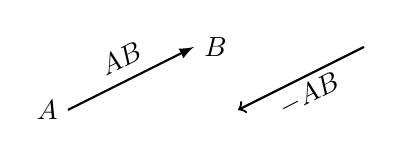
\begin{tikzpicture}[scale=0.8]
\draw[-latex,thick] (0,0) node[left]{$A$}-- (2,1) node[right]{$B$} node[midway,rotate=27,above=1pt]{$\Vj{AB}$};
\draw[<-,thick] (2.7,0) -- (4.7,1)  node[midway,rotate=27,below=-1pt]{$-\Vj{AB}$};
\end{tikzpicture}
}
\end{minipage}}%
\setlength{\ExempleHeight}{\ht\ExempleSaveBox}%
\addtolength{\ExempleHeight}{\dp\ExempleSaveBox}%
\setcounter{exemple}{\SaveExempleCounter}%

\noindent
\begin{minipage}[t]{0.58\linewidth}
\Dfn{
\begin{itemize}
\item la transformation qui laisse tous les points fixes, est appelée translation de \textbf{vecteur nul} $\Vj{0}$.\\
La norme du vecteur nul est 0 mais sa direction et son sens ne sont pas définis.
\item on appelle \textbf{vecteur opposé} au vecteur $\Vj{AB}$ le vecteur noté $-\Vj{AB}$
associé à la translation qui transforme $B$ en $A$. \\
Autrement dit, $-\Vj{AB}=\Vj{BA}$.\\
Le vecteur $-\Vj{AB}$ a donc la même direction et la même norme que $\Vj{AB}$ mais est de sens opposé.
\end{itemize}
}
\end{minipage}%
\hspace{1.2em}
\begin{minipage}[t]{0.38\linewidth}
\Exemple{
\centering
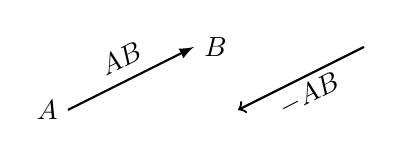
\begin{tikzpicture}[scale=0.8]
\draw[-latex,thick] (0,0) node[left]{$A$}-- (2,1) node[right]{$B$} node[midway,rotate=27,above=1pt]{$\Vj{AB}$};
\draw[<-,thick] (2.7,0) -- (4.7,1)  node[midway,rotate=27,below=-1pt]{$-\Vj{AB}$};
\end{tikzpicture}
% Réponses commentées (pourront resservir, p.ex. pour un corrigé) :
% \smallskip
% \raggedright
% \begin{itemize}
% \item \textcolor{J1}{$\Vj{AA} = \Vj{0}$} (vecteur nul)
% \item \textcolor{J1}{$-\Vj{AB} = \Vj{BA} = \Vj{CD}$} (vecteur opposé)
% \end{itemize}
\rule{0pt}{\dimexpr\DfnHeight-\ExempleHeight\relax}
}
\end{minipage}

\subsection{Interprétation Géométrique}

% Schéma aplati (yscale réduit, au lieu du parallélogramme "carré"
% d'origine) : tient dans le bas de la page 2 sans \newpage, et illustre
% du même coup la remarque "peut être éventuellement plat" juste
% au-dessus. \vspace*{1.5cm} de calage (pensé pour une page neuve)
% retiré : inutile maintenant que le schéma est plus bas et moins haut.
% Boîte Théorème 1 (\Thm, \breakable via CLT2627.sty) rétrécie en la
% plaçant dans une minipage de largeur fixe (15.3cm, au lieu de la pleine
% largeur du cours) : la vidéo Yvan Monka se pose ensuite à côté, hors
% boîte, sur le fond blanc de la page plutôt que sur le fond teinté du
% tcolorbox.
\noindent
\begin{minipage}[t]{15.3cm}
\Thm{\par
\begin{minipage}{10.8cm}
$ABCD$ est un parallélogramme \fbox{si et seulement si} \textcolor{J1}{$\Vj{AB}$ = $\Vj{DC}$}.

\smallskip

Le parallélogramme peut-être éventuellement \og plat\fg{}.

\smallskip

\textbf{Notation : } \textcolor{J1}{on note aussi que cette égalité entraîne $\Vj{AD}=\Vj{BC}$.}
\end{minipage}
\hspace*{0.4cm}
\begin{minipage}{3.4cm}
\centering
% yscale encore réduit (0.55 -> 0.4) pour regagner la place perdue par
% l'ajout de la vidéo (Théorème 1 tenait en bas de page à 0.55 avant
% qu'elle n'arrive) : le schéma est un peu plus aplati mais reste lisible.
\begin{tikzpicture}[yscale=0.3]
\draw[dashed] (1,1) -- (2,3);
\draw[dashed] (4,4) -- (3,2);
\draw[-{Stealth[length=6pt,width=5pt]}, line width=1.6pt] (2,3) -- (4,4);
\draw[-{Stealth[length=6pt,width=5pt]}, line width=1.6pt] (1,1) -- (3,2);
\node[anchor=east, font=\scriptsize] at (1,1) {A};
\node[anchor=north west, font=\scriptsize] at (3,2) {B};
\node[anchor=south east, font=\scriptsize] at (2,3) {D};
\node[anchor=south west, font=\scriptsize] at (4,4) {C};
\end{tikzpicture}
\end{minipage}
}
\end{minipage}
\hspace*{0.3cm}
% Carte vidéo compacte (icône + QR empilés, titre en dessous), sur fond
% blanc à côté de la boîte plutôt que dedans.
\begin{minipage}[t]{3cm}
\centering
{\small\faPlayCircle}\\[3pt]
\ClickableQR{1.4cm}{https://www.youtube.com/watch?v=XokpP_8mTOE&list=PLVUDmbpupCaoKRWtIqAp-FOFSQwftAOtA}\qrcode*[height=1.4cm, level=M]{https://www.youtube.com/watch?v=XokpP_8mTOE&list=PLVUDmbpupCaoKRWtIqAp-FOFSQwftAOtA}\\[3pt]
{\footnotesize\href{https://www.youtube.com/watch?v=XokpP_8mTOE&list=PLVUDmbpupCaoKRWtIqAp-FOFSQwftAOtA}{Utiliser des propri\'et\'es sur les vecteurs}}
\end{minipage}

\bigskip

\begin{center}
{\scriptsize
% Colonnes de difficulté uniformisées à 3.2cm via \cellDiff, comme les
% deux autres tableaux du document (plus de resserrement local à
% 3.4/2.1cm propre à ce tableau-ci). Colonnes 2-4 en type "m" (array) au
% lieu de "p" : centre verticalement les étoiles de l'en-tête (et le
% contenu des lignes Objectif) dans la hauteur réelle de leur ligne,
% plutôt que les caler en haut — utile ici car la ligne d'en-tête serait
% sinon bien plus haute que son contenu réel.
\begin{tabular}{|>{\raggedright\arraybackslash}m{5.2cm}|>{\centering\arraybackslash}m{3.2cm}|>{\centering\arraybackslash}m{3.2cm}|>{\centering\arraybackslash}m{3.2cm}||p{2.1cm}|}
\cline{2-5}
\multicolumn{1}{c|}{} & \headcellV{\starfull{diffgreen}\starempty\starempty} & \headcellV{\starfull{diffblue}\starfull{diffblue}\starempty} & \headcellV{\starfull{diffred}\starfull{diffred}\starfull{diffred}} & \multirow{4}{*}{\parbox{2.1cm}{\centering
% \multirow centre par défaut sur une hauteur de ligne "standard"
% (baselineskip), qui sous-estime fortement la vraie hauteur ici
% (lignes d'objectif multi-lignes très variables) : la carte reste
% collée en haut sans le \vspace ci-dessous, mesuré empiriquement pour
% ce tableau à 4 lignes d'objectif (hauteur totale ~8.15cm, carte
% ~2.7cm) afin de la centrer visuellement.
\vspace{1.8cm}
\href{https://capytale2.ac-paris.fr/web/c/183d-11585990/edn}{\begin{minipage}{2.1cm}\centering
\faLaptop~\textbf{Code Capytale}\\[2pt]
\textbf{D\'efinitions}\\[2pt]
{\ttfamily\bfseries\scriptsize 183d-11585990}
\end{minipage}}\par\smallskip
\textcolor{black}{\qrcode*[height=1.1cm, level=M]{https://capytale2.ac-paris.fr/web/c/183d-11585990/edn}}
}} \\
\cline{1-4}
\cellObj{\textbf{Objectif 1} -- Vecteur $\Vj{MM'}$ associ\'e \`a la translation qui transforme $M$ en $M'$ ; direction, sens et norme} &
\cellDiff[0.16cm]{\IconManuel\ Ex~15 p.183\\\IconFeuilleDeux\ Ex~1, 2} &
\cellDiff[0.16cm]{\IconManuel\ Ex~28 p.184\\\IconManuel\ Ex~30 p.185\\\IconFeuilleDeux\ Ex~3} &
\cellDiff[0.32cm]{\IconFeuilleDeux\ Ex~4} &
\\
\cline{1-4}
\cellObj{\textbf{Objectif 2} -- \'Egalit\'e de deux vecteurs, vecteur nul} &
\cellDiff{\IconManuel\ Ex~18 p.183\\\IconManuel\ Ex~23, 27 p.184\\\IconFeuilleDeux\ Ex~5, 6} &
\cellDiff[0.16cm]{\IconFeuilleDeux\ Ex~7\\\IconManuel\ Ex~31 p.185} &
\cellDiff{\IconManuel\ Ex~35 p.185\\\IconManuel\ Ex~37, 38 p.186\\\IconFeuilleDeux\ Ex~8, 9} &
\\
\cline{1-4}
\cellObj{\textbf{Objectif 3} -- Repr\'esentants d'un vecteur} &
\cellDiff{\IconFeuilleDeux\ Ex~10, 11} &
\cellDiff{\IconFeuilleDeux\ Ex~12} &
\cellDiff{} &
\\
\hline
\end{tabular}
}
\end{center}

\section{Somme de deux vecteurs}

\subsection{Définition et construction bout à bout}

\Dfn{
Soient $\Vj{u}$ et $\Vj{v}$ deux vecteurs. \\
La \textbf{somme} de $\Vj{u}$ et $\Vj{v}$ est le vecteur $\Vj{w}=\Vj{u}+\Vj{v}$ associé
à la translation résultant de l'enchainement des translations de vecteurs $\Vj{u}$ et de vecteur $\Vj{v}$.
}

\medskip

\fbox{\textbf{{\large Méthode de construction bout à bout d'une somme de vecteurs.}}}

% Reconstruit sans multicols/enumerate : deux rangées synchronisées de
% 3 minipages (texte, puis quadrillages) plutôt qu'un enumerate multicol
% à \columnbreak — la rangée de texte peut avoir 3 hauteurs différentes
% (1, 2 ou 3 lignes selon la colonne) sans perturber la rangée de
% quadrillages qui suit, puisqu'elle démarre après la ligne de texte la
% plus haute : les 3 quadrillages s'alignent donc verticalement entre
% eux, quelle que soit la longueur du texte au-dessus. Numéros cerclés
% via \numeroCerne (CLT2627.sty), le même style que produisait
% automatiquement \begin{enumerate} plus haut.
\noindent
\begin{minipage}[t]{5.6cm}
On veut construire la somme des vecteurs $\Vj{u}$ et $\Vj{v}$
\end{minipage}
\hspace*{0.3cm}
\begin{minipage}[t]{5.6cm}
\numeroCerne{1}\ Si l'origine du vecteur somme n'est pas imposée, on choisit un point M quelconque\\
\numeroCerne{2}\ On construit N tel que \\ $\Vj{MN}=\Vj{u}$.
\end{minipage}
\hspace*{0.3cm}
\begin{minipage}[t]{5.6cm}
\numeroCerne{3}\ On construit P tel que $\Vj{NP}=\Vj{v}$. \\
Alors $\boxed{\Vj{u}+\Vj{v}=\Vj{MP}}$.\\[4pt]
\numeroCerne{4}\ On repère en \textcolor{red}{rouge} le vecteur somme et on n'oublie pas de le nommer
\end{minipage}

\medskip

\noindent
\begin{minipage}[t]{5.6cm}
\centering
\begin{tikzpicture}[scale=0.6]
\draw[thin, gray,opacity=0.7] (0,0) grid (6,6);
\draw[-{Stealth},thick,blue] (0,0) node[left]{}--(2,1) node[above]{} node[midway,rotate=30,above]{{\large $\Vj u$}};
\draw[-{Stealth},thick,blue] (2,5)--(4,2) node[right]{} node[midway,rotate=-60,above]{{\large $\Vj v$}};
\end{tikzpicture}
\end{minipage}
\hspace*{0.3cm}
\begin{minipage}[t]{5.6cm}
\centering

\begin{tikzpicture}[scale=0.6]
\draw[thin, gray,opacity=0.7] (0,0) grid (6,6);
%\draw[-{Stealth},very thick,J1, dotted] (1,4) node[left]{$M$}--(3,5) node[above]{$N$} node[midway,rotate=30,above]{{\large $\Vj u$}};
\end{tikzpicture}
\end{minipage}
\hspace*{0.3cm}
\begin{minipage}[t]{5.6cm}
\centering

\begin{tikzpicture}[scale=0.6]
\draw[thin, gray,opacity=0.7] (0,0) grid (6,6);
%\draw[-{Stealth},thick,J1] (1,4) node[left]{$M$}--(3,5) node[above]{$N$} node[midway,rotate=30,above]{{\large $\Vj u$}};
%\draw[-{Stealth},thick,J1, dotted] (3,5)--(5,2) node[right]{$P$} node[midway,rotate=-60,above]{{\large $\Vj v$}};
%\draw[-{Stealth},thick,red, dashed] (1,4)--(5,2) node[midway,rotate=-25,below]{{\large $\Vj u+\Vj v$}};
\end{tikzpicture}
\end{minipage}

\ANoter{L'ordre dans une somme de vecteurs n'a pas d'importance : $\Vj{u}+\Vj{v}=\Vj{v}+\Vj{u}$.}

\Exemple{\par
\begin{minipage}{6.5cm}
Construire le point $D$ \\ tel que $\Vj{ED}=\Vj{BA}+\Vj{CA}$.
\begin{center}
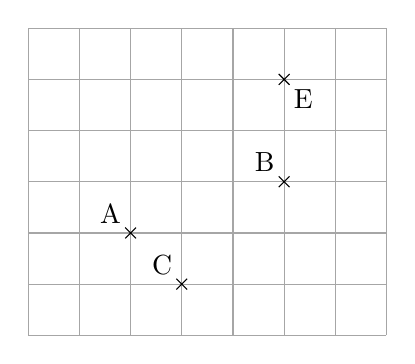
\begin{tikzpicture}[scale=0.65]
\draw[thin, gray,opacity=0.7] (-2,0) grid (5,6);
\draw [ ] (0,2) node[above left]{A} -- ++(-3pt,-3pt) -- ++(6pt,6pt) ++(-6pt,0) -- ++(6pt,-6pt);
\draw [ ] (3,3) node[above left]{B} -- ++(-3pt,-3pt) -- ++(6pt,6pt) ++(-6pt,0) -- ++(6pt,-6pt);
\draw [ ] (1,1) node[above left]{C} -- ++(-3pt,-3pt) -- ++(6pt,6pt) ++(-6pt,0) -- ++(6pt,-6pt);
\draw [ ] (3,5) node[below right]{E} -- ++(-3pt,-3pt) -- ++(6pt,6pt) ++(-6pt,0) -- ++(6pt,-6pt);
% Construction-réponse (segments + point D) : couleur "white" gardée
% (récupérable en repassant "J1") mais opacity=0 en plus, pour une vraie
% invisibilité (sinon le trait blanc reste visible en surimpression sur
% le quadrillage gris derrière) — même principe que le \phantom utilisé
% pour les réponses textuelles ailleurs dans ce document.
\draw[->,thick,white,opacity=0] (3,5)--(0,4) ;
\draw[->,thick,white,opacity=0] (0,4)--(-1,5) ;
\draw [white,opacity=0] (-1,5) node[above right]{D} -- ++(-3pt,-3pt) -- ++(6pt,6pt) ++(-6pt,0) -- ++(6pt,-6pt);
\end{tikzpicture}
\end{center}
\end{minipage}
\hspace*{0.25cm}
\begin{minipage}{6.5cm}
Construire le point $F$ \\ tel que $\Vj{GF}=\Vj{AB}-\Vj{AC}$.
\begin{center}
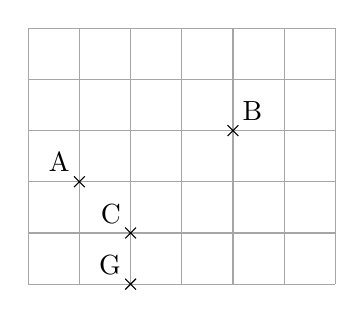
\begin{tikzpicture}[scale=0.65]
\draw[thin, gray,opacity=0.7] (-1,0) grid (5,5);
\draw [ ] (0,2) node[above left]{A} -- ++(-3pt,-3pt) -- ++(6pt,6pt) ++(-6pt,0) -- ++(6pt,-6pt);
\draw [ ] (3,3) node[above right]{B} -- ++(-3pt,-3pt) -- ++(6pt,6pt) ++(-6pt,0) -- ++(6pt,-6pt);
\draw [ ] (1,1) node[above left]{C} -- ++(-3pt,-3pt) -- ++(6pt,6pt) ++(-6pt,0) -- ++(6pt,-6pt);
\draw [ ] (1,0) node[above left]{G} -- ++(-3pt,-3pt) -- ++(6pt,6pt) ++(-6pt,0) -- ++(6pt,-6pt);
\draw[->,thick,white,opacity=0] (1,0)--(4,1) ;
\draw[->,thick,white,opacity=0] (4,1)--(3,2) ;
\draw [white,opacity=0] (3,2) node[above right]{F} -- ++(-3pt,-3pt) -- ++(6pt,6pt) ++(-6pt,0) -- ++(6pt,-6pt);
\end{tikzpicture}
\end{center}
\end{minipage}
\hspace*{0.25cm}
% Carte vidéo compacte, à droite des deux constructions (colonnes D/F
% resserrées à 6.5cm et consignes passées sur 2 lignes pour lui faire
% de la place). \hspace* (et non \hspace) partout dans ce bloc : sinon
% la glue redevient un point de coupure légal pour l'algorithme de
% justification, qui renvoie la carte vidéo à la ligne suivante dès que
% la largeur totale dépasse tant soit peu le \linewidth de l'Exemple.
\begin{minipage}{2.8cm}
\centering
{\small\faPlayCircle}\\[3pt]
\ClickableQR{1.3cm}{https://www.youtube.com/watch?v=nzABUzFM6p8&list=PLVUDmbpupCaoKRWtIqAp-FOFSQwftAOtA}\qrcode*[height=1.3cm, level=M]{https://www.youtube.com/watch?v=nzABUzFM6p8&list=PLVUDmbpupCaoKRWtIqAp-FOFSQwftAOtA}\\[3pt]
{\footnotesize\href{https://www.youtube.com/watch?v=nzABUzFM6p8&list=PLVUDmbpupCaoKRWtIqAp-FOFSQwftAOtA}{Construire un point \`a partir d'une somme de vecteurs}}
\end{minipage}
}

\needspace{10\baselineskip}
\subsection{Relation de Chasles}

\Prp[Relation de Chasles]{\par
\begin{minipage}{10cm}
Soient $A$ et $B$ deux points du plan. Pour tout point $M$, on a :
\[
\Vj{AB}=\Vj{AM}+\Vj{MB}.
\]
\end{minipage}
\hspace{3cm}
\begin{minipage}{5cm}
\begin{tikzpicture}
\draw [ ] (0,0) node[above left]{A} -- ++(-3pt,-3pt) -- ++(6pt,6pt) ++(-6pt,0) -- ++(6pt,-6pt);
\draw [ ] (4,2) node[above left]{B} -- ++(-3pt,-3pt) -- ++(6pt,6pt) ++(-6pt,0) -- ++(6pt,-6pt);
\end{tikzpicture}
\end{minipage}
}

\noindent
\begin{minipage}[c]{0.6\linewidth}
\ANoter{Aller d'Annoville à Brainville, puis de Brainville à Coutances, c'est finalement aller d'Annoville à Coutances.}
\end{minipage}%
\hfill
\begin{minipage}[c]{0.38\linewidth}
\VideoYvanSolo{Appliquer la relation de Chasles}{https://www.youtube.com/watch?v=vqkWtfsCfOo&list=PLVUDmbpupCaoKRWtIqAp-FOFSQwftAOtA}
\end{minipage}

\needspace{12\baselineskip}
\Exemple{
Simplifier les expressions en utilisant la relation de Chasles :
\begin{enumerate}
\item$\Vj{TR}+\Vj{RP}$\\
\phantom{$\Vj{TR}+\Vj{RP} = \Vj{TP}$.}
\medskip
\item$\Vj{GT}+\Vj{AG}$\\
\phantom{$\Vj{GT}+\Vj{AG} = \Vj{AG}+\Vj{GT} = \Vj{AT}$.}
\medskip
\item$\Vj{AB}-\Vj{AC}-\Vj{CB}$\\
\phantom{$\Vj{AB}-\Vj{AC}-\Vj{CB} = \Vj{AB}-(\Vj{AC}+\Vj{CB}) = \Vj{AB}-\Vj{AB} = \Vj{0}$.}
\medskip
\item$\Vj{BC}-\Vj{BA}+\Vj{BD}-\Vj{BC}$\\
\phantom{$\Vj{BC}-\Vj{BA}+\Vj{BD}-\Vj{BC} = \Vj{BD}-\Vj{BA} = \Vj{AD}$.}
\end{enumerate}
}

\subsection{Méthode du parallélogramme}

\fbox{\textbf{{\large Méthode de construction par parallélogramme d'une somme de vecteurs.}}}

\noindent
\begin{minipage}[t]{5.6cm}
On veut construire la somme des vecteurs $\Vj{u}$ et $\Vj{v}$ ayant comme origine commune le point M.
\end{minipage}
\hspace*{0.3cm}
\begin{minipage}[t]{5.6cm}
\numeroCerne{1}\ On repère N et P tels que \\ $\Vj{MN}=\Vj{u}$ et $\Vj{MP}=\Vj{v}$.
\end{minipage}
\hspace*{0.3cm}
\begin{minipage}[t]{5.6cm}
\numeroCerne{2}\ On construit Q tel que MNQP soit un parallélogramme. \\
Alors $\boxed{\Vj{u}+\Vj{v}=\Vj{MQ}}$.
\end{minipage}

\medskip

\noindent
\begin{minipage}[t]{5.6cm}
\centering
\begin{tikzpicture}[scale=0.6]
\draw[thin, gray,opacity=0.7] (0,0) grid (6,6);
\draw[-{Stealth},thick,blue] (1,1)--(3,2) node[midway,rotate=27,below]{{\large $\Vj u$}};
\draw[-{Stealth},thick,blue] (1,1)--(2,4) node[midway,rotate=72,above]{{\large $\Vj v$}};
\node[ptcross] at (1,1) {};
\node[anchor=north east] at (1,1) {M};
\end{tikzpicture}
\end{minipage}
\hspace*{0.3cm}
\begin{minipage}[t]{5.6cm}
\centering
\begin{tikzpicture}[scale=0.6]
\draw[thin, gray,opacity=0.7] (0,0) grid (6,6);
\draw[-{Stealth},thick,blue] (1,1)--(3,2) node[midway,rotate=27,below]{{\large $\Vj u$}};
\draw[-{Stealth},thick,blue] (1,1)--(2,4) node[midway,rotate=72,above]{{\large $\Vj v$}};
\node[ptcross] at (1,1) {};
\node[anchor=north east] at (1,1) {M};
\end{tikzpicture}
\end{minipage}
\hspace*{0.3cm}
\begin{minipage}[t]{5.6cm}
\centering
\begin{tikzpicture}[scale=0.6]
\draw[thin, gray,opacity=0.7] (0,0) grid (6,6);
\draw[-{Stealth},thick,blue] (1,1)--(3,2) node[midway,rotate=27,below]{{\large $\Vj u$}};
\draw[-{Stealth},thick,blue] (1,1)--(2,4) node[midway,rotate=72,above]{{\large $\Vj v$}};
\node[ptcross] at (1,1) {};
\node[anchor=north east] at (1,1) {M};
\end{tikzpicture}
\end{minipage}

\medskip

\begin{center}
{\scriptsize
\begin{tabular}{|>{\raggedright\arraybackslash}m{3.6cm}|>{\centering\arraybackslash}m{4.8cm}|>{\centering\arraybackslash}m{3.2cm}|>{\centering\arraybackslash}m{3.2cm}||p{2.5cm}|}
\cline{2-5}
\multicolumn{1}{c|}{} & \headcellV{\starfull{diffgreen}\starempty\starempty} & \headcellV{\starfull{diffblue}\starfull{diffblue}\starempty} & \headcellV{\starfull{diffred}\starfull{diffred}\starfull{diffred}} & \multirow{2}{*}{\parbox{2.5cm}{\centering
\vspace{0.6cm}
\href{https://capytale2.ac-paris.fr/web/c/b218-11585991/edn}{\begin{minipage}{2.5cm}\centering
\faLaptop~\textbf{Code Capytale}\\[2pt]
\textbf{Somme}\\[2pt]
{\ttfamily\bfseries b218-11585991}
\end{minipage}}\par\smallskip
\textcolor{black}{\qrcode*[height=1.2cm, level=M]{https://capytale2.ac-paris.fr/web/c/b218-11585991/edn}}
\par\rule{0pt}{0.5cm}
}} \\
\cline{1-4}
\cellObjW[0.4cm]{3.6cm}{\textbf{Objectif 4} -- Somme de deux vecteurs et relation de Chasles} &
\cellDiffW{4.8cm}{\IconFeuilleDeux\ Ex~13\\\IconManuel\ Ex~42, 43, 45, 46 p.187\\\IconFeuilleDeux\ Ex~14\\\IconManuel\ Ex~39 p.186 \\ \phantom{RD} } &
\cellDiff[0.16cm]{\IconFeuilleDeux\ Ex~15, 16\\\IconManuel\ Ex~41 p.186} &
\cellDiff[0.32cm]{\IconManuel\ Ex~71 p.192\\\IconManuel\ \faLaptop\ Ex~72, 73 p.192} &
\\
\hline
\end{tabular}
}
\end{center}

\needspace{10\baselineskip}
\section{Multiplication par un scalaire}

% \\ juste après l'accolade ouvrante : ferme la ligne de titre auto-générée
% ("Exemple 6 (introductif) :") avant le \begin{minipage} qui suit, sinon
% ce titre se justifie seul sur toute la largeur de la boîte (gros
% espaces entre les mots) faute de ponctuation de phrase pour le clore.
\Exemple{\\
\begin{minipage}{8cm}
\begin{enumerate}
	\item $\Vj{u}$ est le vecteur
			\begin{itemize}
				\item de même direction que $\Vj{v}$ ;
				\item de même sens que $\Vj{v}$ ;
				\item de norme $3$ fois de celle de $\Vj{v}$.
			\end{itemize}
			On écrit alors : \phantom{$\Vj{u} = 3\Vj{v}$}
	\item $\Vj{j}$ est le vecteur
			\begin{itemize}
				\item de même direction que $\Vj{i}$ ;
				\item de sens opposé à $\Vj{i}$ ;
				\item de norme deux fois celle de $\Vj{i}$.
			\end{itemize}
			On écrit alors : \phantom{$\Vj{j} = -2\Vj{i}$}
\end{enumerate}
\end{minipage}
\hspace{3cm}
\begin{minipage}{8cm}
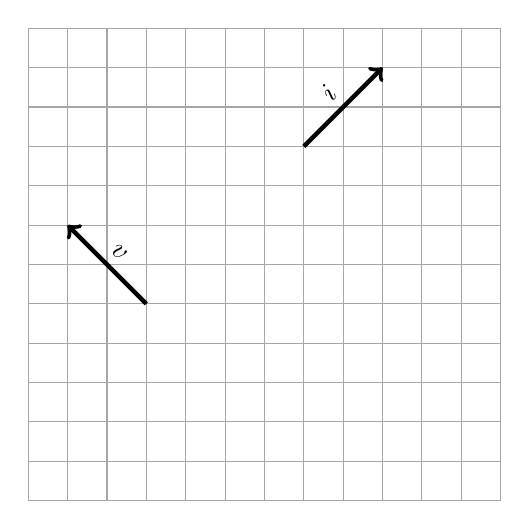
\begin{tikzpicture}[scale=0.5]
\draw[thin,gray,opacity=0.7] (0,0) grid  (12,12);
\draw[->,ultra thick] (3,5)--(1,7) node[midway,rotate=-45,above]{$\Vj v$};
\draw[->,ultra thick,white,opacity=0] (7,5)--(1,11) node[midway,rotate=-45,above]{$\Vj u$};
\draw[->,ultra thick] (7,9)--(9,11) node[midway,rotate=45,above]{$\Vj i$};
\draw[->,ultra thick,white,opacity=0] (11,5)--(7,1) node[midway,rotate=45,above]{$\Vj j$};
\end{tikzpicture}
\end{minipage}
}

% \needspace{10\baselineskip} retiré : empêchait la Définition 6 de
% tenir en bas de la page 4 (elle est \breakable via CLT2627.sty et
% tient largement dans l'espace restant, elle-même needspace déjà
% 4\baselineskip en interne). Boîte rétrécie (minipage 15cm) pour loger
% la vidéo à droite, sur fond blanc ; \\ juste après l'accolade ouvrante
% pour renvoyer le contenu à la ligne suivant le titre "Définition 6 -
% ... :", comme pour \ANoter/\Exemple[introductif] plus haut.
\noindent
\begin{minipage}[t]{15cm}
\Dfn[Produit d'un vecteur par un nombre réel]{\\
Soit $\Vj{u}$ un vecteur non nul et soit $k$ un réel non nul. Alors le vecteur {\Large $\Vj{v}= \textcolor{red}{k}\Vj{u}$} est :
\begin{center}
\begin{tabular}{|p{5cm}|p{5cm}|}
\hline
\centering si $\textcolor{red}{k}>0$ & \centering si $\textcolor{red}{k}<0$\cr
\hline
de même direction que $\Vj{u}$  & de même direction que $\Vj{u}$ \\
de même sens que $\Vj{u}$ & de sens inverse de $\Vj{u}$\\
de norme $k$ fois celle de $\Vj{u}$ & de norme $(-k)$ fois celle de $\Vj{u}$\\
\hline
\end{tabular}
\end{center}
}
\end{minipage}
\hspace*{0.3cm}
\begin{minipage}[t]{3cm}
\centering
{\small\faPlayCircle}\\[3pt]
\ClickableQR{1.4cm}{https://www.youtube.com/watch?v=ak1WcdhOaFA&list=PLVUDmbpupCaoKRWtIqAp-FOFSQwftAOtA}\qrcode*[height=1.4cm, level=M]{https://www.youtube.com/watch?v=ak1WcdhOaFA&list=PLVUDmbpupCaoKRWtIqAp-FOFSQwftAOtA}\\[3pt]
{\footnotesize\href{https://www.youtube.com/watch?v=ak1WcdhOaFA&list=PLVUDmbpupCaoKRWtIqAp-FOFSQwftAOtA}{Construire un vecteur comme produit et somme de vecteurs}}
\end{minipage}

\needspace{20\baselineskip}
\Exemple{

\begin{enumerate}
\item Exprimer le vecteur $\Vj{AC}$ en fonction du vecteur $\Vj{AB}$ dans chacun des cas suivants :
\\[0.5em]
\begin{tabular}{p{0.5\textwidth} p{0.5\textwidth}}
\begin{tikzpicture}[x=1.5cm, y=1cm, >=stealth]
    \draw (-0.5,0) -- (2.5,0);
    \foreach \x in {-0.5,0,...,2.5} {
        \draw (\x, 0.08) -- (\x, -0.08);
    }
    \node[ptcross] at (0,0) {};
    \node[anchor=south,yshift=2pt] at (0,0) {$A$};
    \node[ptcross] at (1,0) {};
    \node[anchor=south,yshift=2pt] at (1,0) {$B$};
    \node[ptcross] at (2,0) {};
    \node[anchor=south,yshift=2pt] at (2,0) {$C$};
    \node at (1,-0.6) {\phantom{$\Vj{AC}=2\Vj{AB}$}};
\end{tikzpicture}
&
\begin{tikzpicture}[x=1.5cm, y=1cm, >=stealth]
    \draw (-2,0) -- (2,0);
    \foreach \x in {-2,-1.5,...,2} {
        \draw (\x, 0.08) -- (\x, -0.08);
    }
    \node[ptcross] at (1,0) {};
    \node[anchor=south,yshift=2pt] at (1,0) {$A$};
    \node[ptcross] at (1.5,0) {};
    \node[anchor=south,yshift=2pt] at (1.5,0) {$B$};
    \node[ptcross] at (-1.5,0) {};
    \node[anchor=south,yshift=2pt] at (-1.5,0) {$C$};
    \node at (0,-0.6) {\phantom{$\Vj{AC}=-5\Vj{AB}$}};
\end{tikzpicture}
\end{tabular}

\vspace{2cm}

\item Dans chacun des cas suivants, représenter le vecteur $\Vj{AC}$ tel que :
\\[0.5em]
\begin{tabular}{p{0.5\textwidth} p{0.5\textwidth}}
 $\Vj{AC} = -3\Vj{AB}$ & $\Vj{AC} = \dfrac{1}{3}\Vj{AB}$ \\[1em]
\begin{tikzpicture}[x=1.2cm, y=1cm, >=stealth]
    \draw (-2,0) -- (2.5,0);
    \foreach \x in {-2,-1.5,...,2.5} {
        \draw (\x, 0.08) -- (\x, -0.08);
    }
    \node[ptcross] at (0,0) {};
    \node[anchor=south,yshift=2pt] at (0,0) {$A$};
    \node[ptcross] at (0.5,0) {};
    \node[anchor=south,yshift=2pt] at (0.5,0) {$B$};
    \node[ptcross,white,opacity=0] at (-1.5,0) {};
    \node[anchor=south,yshift=2pt,white,opacity=0] at (-1.5,0) {\phantom{$C$}};
\end{tikzpicture}
&
\begin{tikzpicture}[x=1.2cm, y=1cm, >=stealth]
    \draw (-1.5,0) -- (2.5,0);
    \foreach \x in {-1.5,-1,...,2.5} {
        \draw (\x, 0.08) -- (\x, -0.08);
    }
    \node[ptcross] at (0,0) {};
    \node[anchor=south,yshift=2pt] at (0,0) {$A$};
    \node[ptcross] at (1.5,0) {};
    \node[anchor=south,yshift=2pt] at (1.5,0) {$B$};
    \node[ptcross,white,opacity=0] at (0.5,0) {};
    \node[anchor=south,yshift=2pt,white,opacity=0] at (0.5,0) {\phantom{$C$}};
\end{tikzpicture}
\end{tabular}

\vspace{3cm}

\end{enumerate}
}

\newpage
\Exemple{\\
\noindent
\begin{minipage}[t]{9.2cm}
\numeroCerne{1}\ Placer les points H, I et J tels que :\\
(a) $\Vj{AH}=\dfrac53\Vj{AB}$\ \hfill (b) $\Vj{BI}=\dfrac23\Vj{BC}$\ \hfill  (c) $\Vj{DJ}=\dfrac58\Vj{DC}$

\begin{center}
\begin{tikzpicture}[scale=0.55]
\draw[thin,gray,opacity=0.5] (0,0) grid (10,6);
\draw[very thick,magenta] (3,5) -- (6,5) -- (9,2) -- (1,1) -- cycle;
\node[ptcross] at (3,5) {};
\node[anchor=south] at (3,5) {\textsf{A}};
\node[ptcross] at (4,5) {};
\node[anchor=south] at (4,5) {\textsf{E}};
\node[ptcross] at (6,5) {};
\node[anchor=south] at (6,5) {\textsf{B}};
\node[ptcross] at (9,2) {};
\node[anchor=west] at (9,2) {\textsf{C}};
\node[ptcross] at (1,1) {};
\node[anchor=north east] at (1,1) {\textsf{D}};
\node[ptcross] at (2,3) {};
\node[anchor=east] at (2,3) {\textsf{F}};
\node[ptcross,white,opacity=0] at (8,5) {};
\node[anchor=south,white,opacity=0] at (8,5) {\textsf{\phantom{H}}};
\node[ptcross,white,opacity=0] at (8,3) {};
\node[anchor=west,white,opacity=0] at (8,3) {\textsf{\phantom{I}}};
\node[ptcross,white,opacity=0] at (6,1.625) {};
\node[anchor=south,white,opacity=0] at (6,1.625) {\textsf{\phantom{J}}};
\end{tikzpicture}
\end{center}
\end{minipage}
\hfill
\begin{minipage}[t]{7cm}
\numeroCerne{2}\ Construire dans la figure ci-dessous des représentants des vecteurs $2\Vj{u}$, $-\Vj{u}$ et $\dfrac12\Vj{u}$ :

\begin{center}
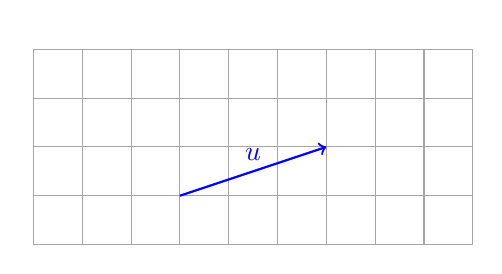
\begin{tikzpicture}[scale=0.62]
\draw[thin,gray,opacity=0.7] (-3,-1) grid (6,3);
\draw[->,thick,blue] (0,0) -- (3,1) node[midway,above]{$\Vj{u}$};
\draw[->,thick,white,opacity=0] (-2,-1) -- (4,1) node[midway,rotate=20,above]{$2\Vj{u}$};
\draw[->,thick,white,opacity=0] (2,3) -- (-1,2) node[midway,rotate=20,above]{$-\Vj{u}$};
\draw[->,thick,white,opacity=0] (-3,2) -- (-1.5,2.5) node[midway,rotate=20,above]{$\frac12\Vj{u}$};
\end{tikzpicture}
\end{center}
\end{minipage}
}

\section{Vecteurs colinéaires}

% needspace retiré (au lieu de 16\baselineskip) : la Définition 7 et
% l'Exemple 8 (quadrillage réduit à scale=0.5) tiennent tous les deux en
% bas de la page 5 sans lui, alors qu'un seuil trop haut les renvoyait
% en bloc page 6 malgré la place restante.
\noindent
\begin{minipage}[t]{0.55\linewidth}
\Dfn[Vecteurs colinéaires]{\par
Deux vecteurs $\Vj{u}$ et $\Vj{v}$ sont dit \textbf{colinéaires} s'il existe un réel $k$ tel que $\Vj{v}=k\Vj{u}$ ou $\Vj{u}=k\Vj{v}$.
}
\end{minipage}%
\hspace{1.2em}
\begin{minipage}[t]{0.40\linewidth}
\Exemple{\par
\centering
\begin{tikzpicture}[scale=0.5]
\draw[thin,gray,opacity=0.5] (0,0) grid (6,4);
\draw[->,thick,blue] (1,3) -- (3,4) node[midway,above]{$\Vj u$};
\draw[->,thick,J1] (5,3) -- (1,1) node[midway,above]{$\Vj v$};
\end{tikzpicture}

\smallskip
\raggedright
\phantom{$\Vj{v} = -2\Vj{u}$}\\
%, donc $\Vj{u}$ et $\Vj{v}$ sont colinéaires.
}
\end{minipage}

\medskip

\ANoter{
\begin{itemize}
\item deux vecteurs sont colinéaires si et seulement s'ils ont \textbf{même direction}.
\item le vecteur nul est colinéaire à n'importe quel vecteur. En effet, $\Vj{0}=0\Vj{u}$.
\item la notion de colinéarité est fortement liée à celle de parallélisme et d'alignement.
\end{itemize}
}

\Prp[Colinéarité et parallélisme]{
\begin{spacing}{1.7}
Soient A, B, C et D quatre points.

\medskip

Les vecteurs $\Vj{AB}$ et $\Vj{CD}$ sont colinéaires \fbox{si et seulement si} les droites (AB) et (CD) sont \textcolor{J1}{parallèles (ou confondues)}.
\end{spacing}
}

\Exemple{\\
\begin{minipage}{6cm}
\begin{tikzpicture}[scale=0.7]
\draw[thin,gray,opacity=0.5] (0,0) grid (8,5);
\draw[|-{Stealth[length=10pt,inset=2pt]},very thick,airforceblue] (1,2) node[below=2pt]{A} --(2,4) node[above=2pt]{B} node[midway,rotate=60,above=2pt]{$\Vj{AB}$};
\draw[dotted,red, thick](0,0) -- (1,2);
\draw[dotted,red, thick](2,4) --(2.5,5) ;
\draw[|-{Stealth[length=10pt,inset=2pt]},very thick,airforceblue] (6,5) node[below right]{C} --(4,1) node[below=2pt]{D} node[midway,rotate=60,above=2pt]{$\Vj{CD}$};
\draw[dotted,red](3.5,0) -- (4,1);
\end{tikzpicture}
\end{minipage}
\hspace{0.5cm}
\begin{minipage}{12cm}
\textbf{Rédaction : }

\vspace*{3cm}

%Ici, on a : $\Vj{CD} = \textcolor{J1}{-2} \  \Vj{AB}$ donc $\Vj{AB}$ et $\Vj{CD}$ sont \textcolor{J1}{colinéaires}.

\medskip

%Ainsi : les droites \textcolor{J1}{$(AB)$} et \textcolor{J1}{$(CD)$} sont \textcolor{J1}{parallèles}.
\end{minipage}
}

\needspace{12\baselineskip}
\Prp[Colinéarité et alignement]{
\begin{spacing}{1.7}
Soient A, B et C trois points distincts.

\medskip

Les points A, B et C sont alignés \fbox{si et seulement si} les vecteurs $\Vj{AB}$ et $\Vj{AC}$ sont \textcolor{J1}{colinéaires}.
\end{spacing}
}

\Exemple{\\
\begin{minipage}{10cm}
%\textbf{Rédaction : }

\vspace*{0.5cm}

Ici, on a : $\Vj{AB} = \dfrac35 \  \Vj{AC}$ donc \textcolor{J1}{$\Vj{AB}$} et \textcolor{J1}{$\Vj{AC}$} sont \textcolor{J1}{colinéaires}.

\medskip

Ainsi : \textcolor{J1}{les points A, B et C sont alignés.}
\end{minipage}
\hspace{1cm}
\begin{minipage}{6cm}
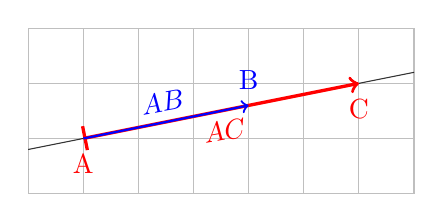
\begin{tikzpicture}[scale=0.7]
\draw[thin,gray,opacity=0.5] (0,1) grid (7,4);
\draw[opacity=0.8](0,1.8) --(7,3.2) ;
\draw[|->,very thick,red] (1,2) node[below=2pt]{A} --(6,3) node[below=2pt]{C} node[midway,rotate=10,below]{$\Vj{AC}$};
\draw[->, thick,blue] (1,2) --(4,2.6) node[above=2pt]{B} node[midway,rotate=10,above]{$\Vj{AB}$};
\end{tikzpicture}
\end{minipage}
}

% 3 vidéos "exercice" (celle sur l'égalité vectorielle exploite à la
% fois la somme, Objectif 4, et la colinéarité, Objectif 5 : posée ici
% plutôt que près du Théorème 1, pour rester après les deux notions
% qu'elle mobilise), regroupées sur 3 colonnes sans bordures plutôt
% qu'empilées en \VideosYvanMonka — intitulés simplifiés (plus de
% préfixe "EXERCICE :", vidéos de cours correspondantes retirées).
% 3 minipages plutôt qu'un vrai tabular : le "&" des url YouTube
% (?v=...&list=...) est un caractère actif (séparateur de colonne) dans
% un tabular, il casserait la compilation.
\begin{center}
\begin{minipage}{5.5cm}\VideoCardCell{D\'emontrer que deux vecteurs sont colin\'eaires}{https://www.youtube.com/watch?v=62Uh6UKz-Wk&list=PLVUDmbpupCaoKRWtIqAp-FOFSQwftAOtA}\end{minipage}%
\hfill
\begin{minipage}{5.5cm}\VideoCardCell{Construire un point \`a partir d'une \'egalit\'e vectorielle}{https://www.youtube.com/watch?v=1C6KEwbO-b8&list=PLVUDmbpupCaoKRWtIqAp-FOFSQwftAOtA}\end{minipage}%
\hfill
\begin{minipage}{5.5cm}\VideoCardCell{Exprimer un vecteur en fonction de deux autres}{https://www.youtube.com/watch?v=ODZGKdIKewo&list=PLVUDmbpupCaoKRWtIqAp-FOFSQwftAOtA}\end{minipage}
\end{center}

\bigskip

\begin{center}
{\scriptsize
\begin{tabular}{|>{\raggedright\arraybackslash}m{5.2cm}|>{\centering\arraybackslash}m{3.2cm}|>{\centering\arraybackslash}m{3.2cm}|>{\centering\arraybackslash}m{3.2cm}||p{2.5cm}|}
\cline{2-5}
\multicolumn{1}{c|}{} & \headcellV{\starfull{diffgreen}\starempty\starempty} & \headcellV{\starfull{diffblue}\starfull{diffblue}\starempty} & \headcellV{\starfull{diffred}\starfull{diffred}\starfull{diffred}} & \multirow{3}{*}{\parbox{2.5cm}{\centering
% Même correctif que pour le 1er tableau, valeur plus petite (tableau à
% 2 lignes d'objectif, donc moins de hauteur à combler).
\vspace{1.2cm}
\href{https://capytale2.ac-paris.fr/web/c/bd09-11585993/edn}{\begin{minipage}{2.5cm}\centering
\faLaptop~\textbf{Code Capytale}\\[2pt]
\textbf{Colin\'earit\'e}\\[2pt]
{\ttfamily\bfseries bd09-11585993}
\end{minipage}}\par\smallskip
\textcolor{black}{\qrcode*[height=1.2cm, level=M]{https://capytale2.ac-paris.fr/web/c/bd09-11585993/edn}}
}} \\
\cline{1-4}
\cellObj{\textbf{Objectif 5} -- Produit d'un vecteur par un nombre r\'eel et colin\'earit\'e de deux vecteurs} &
\cellDiff{\IconFeuilleTrois\ Ex~1, 2\\\IconManuel\ Ex~18, 19 p.207\\\IconManuel\ Ex~41, 42 p.208} &
\cellDiff[0.32cm]{\IconFeuilleTrois\ Ex~3 \\ \IconManuel\ Ex~43, 44 p.209} &
\cellDiff{} &
\\
\cline{1-4}
\cellObj[0.32cm]{\textbf{Objectif 6} -- D\'ecomposition d'un vecteur en fonction de deux vecteurs non colin\'eaires} &
\cellDiff[0.32cm]{\IconFeuilleTrois\ Ex~4, 5} &
\cellDiff[0.16cm]{\IconFeuilleTrois\ Ex~6, 7\\\IconManuel\ Ex~45 p.209 \\ \IconManuel\  74 p.212} &
\cellDiff[0.16cm]{\IconFeuilleTrois\ Ex~8\\ \IconManuel\ Ex~75, 78 p.212} &
\\
\hline
\end{tabular}
}
\end{center}

\bigskip

% Vidéos de révision globale du chapitre (plutôt qu'en tête de document) :
% regroupées ici, tout à la fin, une fois toutes les notions vues.
\VideosYvanMonka{LE COURS : Les vecteurs (r\'evision compl\`ete)}{https://www.youtube.com/watch?v=aSSDBNn_rRI&list=PLVUDmbpupCaoKRWtIqAp-FOFSQwftAOtA}{QCM : Les vecteurs (auto-\'evaluation)}{https://www.youtube.com/watch?v=AwzchpN8S9g&list=PLVUDmbpupCaoKRWtIqAp-FOFSQwftAOtA}

\end{document}
